\chapter{Sistemi \ac{RADAR}}
Diversamente dal sistema di trasmissione analogica utilizzato per trasmettere informazione in un segnale da far giungere da una sorgente ad un destinatario quanto più fedelmente possibile, un sistema \acf{RADAR} ha lo scopo individuare un bersaglio inviando un segnale e ricevendo un eco che ne consenta l'individuazione, calcolandone la distanza, la direzione e lo spostamento.

\begin{figure}[ht]\centering
	\begin{tikzpicture}
	\draw (0,3) pic[rotate=10]{antenna} --++(0,-.5)--++(-.5,-1)++(.5,1)--++(.5,-1)++(-.5,0) node[below]{RADAR};
	\draw (6,4) circle(3pt)node[right,outer sep=3pt]{bersaglio};
	\draw [decorate,decoration={expanding waves,angle=3}] (6,4)--(3,3.5);
	\end{tikzpicture}
	\caption{Sistema \ac{RADAR} con una antenna ricetrasmittente}
	\label{fig:radar_tx_rx}
\end{figure}

\section{Sistema RADAR}\index{RADAR}
L'antenna emette un segnale con una potenza di trasmissione $P_T$. La densità di potenza per unità di superficie che incide su un bersaglio a distanza $R$ è
\begin{equation}
\frac{P_T G_T}{4\pi R^2}
\end{equation}
Parte del segnale si riflette sul bersaglio in proporzione alla sua \keyword[RADAR!sezione RADAR]{sezione RADAR} rilevabile $\sigma [\si{\square\meter}]$ che ingloba anche la direttività dell'“antenna” bersaglio. Della potenza riflessa giunge al ricevutore la quota parte intercettabile dall'area efficace $A_R$ dell'antenna ricevente, attenuata per la divergenza sferica pari al fattore $1/4\pi R^2$. Il sistema ricevitore deve riconoscere il segnale inviato che si è notevolmente attenuato in proporzione inversa alla quarta potenza della distanza $1/R^4$ che è ricevuto con una potenza
\begin{equation}
P_R = \frac{P_T G_T}{4\pi R^2}\,\sigma\,\frac{A_R}{4\pi R^2}
\end{equation}
Elaborando il segnale con un demodulatore d'ampiezza si determina se la potenza ricevuta supera una soglia: dal tempo  $\tau$ intercorso tra l'invio del segnale e il suo ritorno è possibile stimare la distanza del bersaglio $R=c\,\tau/2$, considerando una velocità di propagazione del fronte d'onda pari alla velocità della luce $c$. Il \ac{RADAR} attende un tempo massimo $t_p$ prima di emettere un nuovo impulso, per cui resta definito il massimo raggio di visibilità dei bersagli $R_\text{max}=c\frac{t_p}{2}$.

\begin{nota}In un \ac{RADAR} usualmente si usa la stessa antenna per trasmettere e ricevere potendo disaccoppiare il segnale trasmesso da quello ricevuto.\end{nota}

L'apparecchiatura ricevente è costituita dall'antenna affetta dal rumore del canale radio, da un blocco filtro passa basso, da un demodulatore d'ampiezza a inviluppo che misura l'ampiezza del segnale, da un blocco decisore impostato su una soglia.
\begin{figure}[ht]
\centering
\begin{tikzpicture}[>=latex',
start chain=going right,
node distance=5mm,
every node/.style={on chain,rounded corners=1mm},
every join/.style={->},
block/.style={draw,align=center,text width=2.5cm}]
\pic[rotate=180,on chain,join]{antennarx};
\coordinate[join,on chain](start);
\node[sum,on chain,join]{$+$};
\begin{scope}[start branch=above, every join/.style={<-},]
\node[on chain=going above,join]{$n(t)$};
\end{scope}
\node[block,join]{Filtro Passa Banda $H(f)$};
\node[block,join]{Demodulatore AM a inviluppo};
\node[block,join]{Decisore a soglia};
\coordinate[join](end);
\end{tikzpicture}
\caption{Schema a blocchi di ricevitore \ac{RADAR}}
\label{fig:ricevitore_radar}
\end{figure}

\section{Risoluzione radiometrica}\index{risoluzione radiometrica}
L'obiettivo del dimensionamento di un sistema \ac{RADAR} è di ottimizzare la potenza trasmissibile e la struttura dell'antenna per ottenere la massima capacità di distinguere il segnale dell'eco riflesso dal rumore.

Data la massima distanza $R_\text{max}$ a cui si vuole rilevare un bersaglio con sezione \ac{RADAR} $\sigma_\text{min}$ si calcola il rapporto segnale rumore che garantisca una minima probabilità di mancato bersaglio e di falso allarme. Non è possibile realizzare \ac{RADAR} in grado di rilevare un qualsiasi bersaglio a qualsiasi distanza.

Per migliorare il rapporto segnale rumore si può aumentare la potenza trasmessa e l'area efficace dell'antenna ma è possibile massimizzare tale rapporto grazie alla teoria dei segnali.

In assenza di bersaglio non vi è il segnale riflesso, in ingresso al ricevitore si ha esclusivamente rumore gaussiano bianco $n(t)$.
In presenza del bersaglio si otterrà una replica del segnale trasmesso attenuata e ritardata nel tempo in proporzione alla distanza, quindi un segnale $s_R(t)=k\cdot s_T(t-\tau)$ a cui si somma il rumore $n(t)$.

Il demodulatore non può essere coerente perché non può conoscere la fase del segnale ricevuto data la distanza incognita. Si utilizza pertanto un demodulatore ad inviluppo che fornisce l'ampiezza del segnale estraendo le componenti in fase e in quadratura, del segnale e del rumore:
\begin{equation}
s_R(t)=s_R^\text{I}(t)\cos{\omega_0 t}-s_R^\text{Q}(t)\cos{\omega_0 t}=A(t)\cos{\omega_0 t+\phi(t)}\quad A(t)=\sqrt{s_R^\text{I}(t)+s_R^\text{Q}(t)}
\end{equation}
\begin{equation}
n(t)=n^\text{I}(t)\cos{\omega_0 t}-n^\text{Q}(t)\cos{\omega_0 t}=r(t)\cos{\omega_0 t+\phi(t)}\quad r(t)=\sqrt{n^\text{I}(t)+n^\text{Q}(t)}
\end{equation}

Essendo il rumore la composizione di due variabili aleatorie gaussiane si ottiene una densità di probabilità di variabile aleatoria di Rayleigh (v.\ref{eq:Rayleigh}). 

In assenza di bersaglio la probabilità di rilevare una tensione all'uscita del demodulatore ad inviluppo superiore alla soglia è la \keyword[probabilità!di falso allarme]{probabilità di falso allarme} $P_\text{FA}$ (v.\ref{fig:radar_prob_falso_allarme}).

In presenza di bersaglio ricevo il segnale riflesso cui si somma il rumore per cui il demodulatore ha in ingresso il segnale
\begin{equation}
A(t)\cos{\omega_0 t+\phi(t)}+r(t)\cos{\omega_0 t+\phi(t)}=D(t)\cos{\omega_0 t+\phi(t)}
\end{equation}
di cui il demodulatore estrarrà il modulo $D(t)$, pari al modulo della somma dei vettori rotanti del segnale e del rumore. 

Nel funzionamento nominale del \ac{RADAR} il termine del segnale è dominante sul rumore (v.fig.\ref{fig:segnale_modulato_angolarmente_affetto_da_rumore}), si può approssimare il modulo con la somma delle componenti in fase, considerando l'errore di fase uniformente distribuito in $[0,2\pi]$:
\[D(t)\cong A(t)+r(t)\cos{\phi_N(t)-\phi(t)}\cong A(t)+r(t)\cos{\phi_N(t)}\]

Il modulo del segnale ricevuto avrà approssimativamente una statistica gaussiana con il valore medio dipendente dalla potenza dell'eco che ritorna al ricevitore: maggiore è la potenza ritornata maggiore sarà la tensione all'uscita del demodulatore. Un valore di tensione al demodulatore sotto la soglia si verifica con una certa \keyword[probabilità!di bersaglio mancato]{probabilità di bersaglio mancato}.

La scelta del valore di soglia è un compromesso tra una bassa probabilità di bersaglio mancato e una bassa probabilità di falso allarme. Il valore di soglia ottimo, che determina la probabilità di falso allarme e bersaglio mancato, è influenzato dalla varianza del rumore gaussiano e assieme ai parametri di progetto, la sezione \ac{RADAR} minima $\sigma_\text{min}$ e la distanza massima di rilevazione $R_\text{max}$, si determina la potenza da trasmettere tale che il rapporto segnale rumore \ac{SNR} garantisca che la potenza dell'eco ricevuto sia sufficientemente grande rispetto alla potenza del rumore.
Il dimensionamento del sistema con i parametri $\sigma_\text{min},R_\text{max},P_\text{FA},P_\text{BM}$ segue il criterio di \emph{Neymann-Pearson}.

\begin{figure}[ht!]\centering\def\soglia{5}
	\subfloat[Probabilità di falso allarme]{\begin{tikzpicture}
		\begin{axis}[xlabel=$X$,ylabel=$f_R(X)$,ytick=\empty,xtick={5.0},xticklabels={soglia},yticklabels={},yscale=.9,domain=0:10]
		\addplot [name path=rayleigh5,smooth]{x/5.*exp(-(x^2)/10.)};
		\path[name path=axis] (axis cs:0,0)--node[above right,pin=45:$P_\text{FA}$]{}(axis cs:10,0);
		\addplot[pattern=north west lines] fill between[of=rayleigh5 and axis,soft clip={domain=\soglia:10}];
		\end{axis}
		\label{fig:radar_prob_falso_allarme}
		\end{tikzpicture}
	}\quad\subfloat[Probabilità di bersaglio mancato]{
		\begin{tikzpicture}
		\begin{axis}[xlabel=$X$,ylabel=$f_D(X)$,xtick={10},ytick=\empty,xticklabels={A},yticklabels={},yscale=.9,extra x ticks={5.0},extra x tick labels={soglia},extra x tick style={grid=major},domain=0:20]
		\addplot [name path=gauss5,smooth] {100*gauss(x,10,5)};
		\path[name path=axis] (axis cs:0,0.75)--node[above right,pos=.33,pin=135:$P_\text{BM}$]{}(axis cs:\soglia,.75);
		\addplot[pattern=north east lines] fill between[of=gauss5 and axis,soft clip={domain=0:\soglia}];
		\end{axis}
		\label{fig:radar_prob_bersaglio_mancato}
		\end{tikzpicture}
	}\quad\subfloat[Valore di soglia]{
		\begin{tikzpicture}
		\begin{axis}[xscale=1.3,xlabel=$X$,xtick=\empty,ytick=\empty,xticklabels={},extra x ticks={5.0},extra x tick labels={soglia},extra x tick style={grid=major},yscale=.8,domain=0:20]
		\addplot [name path=gauss5,smooth] {gauss(x,10,5)};
		\addplot [name path=rayleigh5,smooth]{x/5.*exp(-(x^2)/10.)};
		\path[name path=axis] (axis cs:0,0)--node[above right,pos=.25,pin=45:$P_\text{FA}$]{}node[above left,pos=.25,pin=135:$P_\text{BM}$]{}(axis cs:20,0);
		\addplot[pattern=north west lines] fill between[of=rayleigh5 and axis,soft clip={domain=\soglia:20}];
		\addplot[pattern=north east lines] fill between[of=gauss5 and axis,soft clip={domain=0:\soglia}];
		\end{axis}
		\end{tikzpicture}
	}
\label{fig:radar_soglia}
\end{figure}

Per ottimizzare la potenza di picco del segnale ricevuto bisogna agire sulla funzione di trasferimento $H(f)$ del filtro passa banda del ricevitore. Per massimizzare il valore di uscita del demodulatore in presenza di bersaglio bisogna esaltare la potenza di picco del segnale, nell'istante $t_m$ del suo massimo, più della potenza del rumore, agendo sulla funzione di trasferimento del filtro che viene adattata al segnale trasmesso. 

Data la trasformata di Fourier del segnale ricevuto $k s(t-\tau) \stackrel{\Fourier}{\longrightarrow} k S(f) \e{-\jmath\omega_0\tau}$ si calcola la potenza di picco del segnale nell'istante $t_m$:
\begin{equation}
P_S^\text{PP}=\abs{\intinf{k S(f)\e{-\jmath\omega_0 \tau} H(f)\e{\jmath\omega_0 t_m}}{f}}^2
\end{equation}
e la potenza media del rumore (a banda stretta)
\begin{equation}
P_N=\intinf{h_n\abs{H(f)}^2}{f}
\end{equation}

Il rapporto segnale rumore, definito come rapporto della potenza picco-picco del segnale e la potenza media del rumore, risulta
\begin{equation}\begin{split}
\restrict{\frac{S}{N}}{\text{post dem}}&=\frac{P_S^\text{PP}}{P_N}=\frac{\abs{\intinf{k S(f) H(f)\e{\jmath\omega_0 (t_m-\tau)}}{f}}^2}{\intinf{h_n\abs{H(f)}^2}{f}}=
\frac{\intinf{k^2\abs{S(f)}^2\abs{H(f)}^2}{f}}{\intinf{h_n\abs{H(f)}^2}{f}}=\\
&<\frac{\intinf{k^2\abs{S(f)}^2}{f}\cdot\intinf{\abs{H(f)}^2}{f}}{h_n\intinf{\abs{H(f)}^2}{f}}=\frac{\intinf{k^2\abs{S(f)}^2}{f}}{h_n}=\frac{E_R}{h_n}
\end{split}\end{equation} 

Per il teorema di Parseval (v.eq.\ref{eq:parseval}) il termine a numeratore $E_R=\intinf{\abs{k S(f)}^2}{f}$ è l'energia del segnale ricevuto.

Il rapporto segnale rumore è maggiorato dall'energia del segnale ricevuto rapportata alla densità spettrale di rumore gaussiano bianco.

L'uguaglianza si ha per \keyword[filtro adattato]{filtro adattato} ovvero con spettro\footnote{Il filtro adattato opera il rifasamento di tutte le componenti spettrali.} \begin{equation}H(f)\propto\conj{S}(f)\label{eq:radar_filtro_adattato_rumore_bianco}\end{equation}

Il filtro adattato massimizza il rapporto segnale rumore ottenendo la massima autocorrelazione tra segnale ricevuto e filtro nell'istante $\tau=t_m$
\begin{equation}\begin{split}
\restrict{\frac{S}{N}}{\text{post dem}}&=\dfrac{\abs{\intinf{k\alpha\abs{S(f)}^2\e{\jmath\omega_0(t_m-\tau)}}{f}}^2}{h_n\intinf{\alpha^2\abs{S(f)}^2}{f}}=\dfrac{\alpha^2 k^2\abs{\intinf{\abs{S(f)}^2\e{\jmath\omega_0(t_m-\tau)}}{f}}^2}{\alpha^2 h_n\intinf{\abs{S(f)}^2}{f}}=\\
&=\frac{k^2\intinf{\abs{S(f)}^2}{f}}{h_n}=\frac{E_R}{h_n}
\end{split}\end{equation}

In caso di rumore gaussiano non bianco è necessario pesare in misura maggiore le componenti che hanno un rapporto più grande possibile tra ampiezza dello spettro del segnale e ampiezza dello spettro del rumore.
\begin{equation}
H(f)\propto\frac{\conj{S}(f)}{h'_n}
\label{eq:radar_filtro_adattato_rumore_colorato}
\end{equation}

\section{Risoluzione geometrica azimutale}\index{risoluzione geometrica azimutale}
Un sistema \ac{RADAR} con una antenna omnidirezionale può rilevare la presenza di un bersaglio e calcolare la sua distanza che è proporzionale al ritardo col quale l'eco torna all'antenna
\begin{equation}
R=c\,\frac{\tau}{2}
\end{equation}

Per poter determinare la direzione da cui proviene il segnale riflesso una antenna direzionale viene fatta ruotare sul proprio asse per spazzare lo spazio aereo con un fascio di radiazioni ristretto in un piano azimutale in cui è concentrata la potenza trasmessa dal \ac{RADAR}.

\newcommand{\radar}{
\pgfmathparse{\targetlong-\waveazimutalfov/2}\let\longmin=\pgfmathresult
\pgfmathparse{\targetlong+\waveazimutalfov/2}\let\longmax=\pgfmathresult
\pgfmathparse{\longmin+\longstep}\let\longfor=\pgfmathresult
\pgfmathparse{\longmax-\longstep}\let\longlast=\pgfmathresult
\pgfmathparse{\latmin+\latstep}\let\latfor=\pgfmathresult
\pgfmathparse{\latmax-\latstep}\let\latlast=\pgfmathresult
\begin{tikzpicture}[x={(1cm,0)},y={(-.5cm,-.5cm)},z={(0cm,1cm)}]% sistema di riferimento 3D

% piano di base
\draw [help lines](-4,-3,0)--(-4,3,0)--(4,3,0)--(4,-3,0)--cycle;

% draw base circle in plane xy and axis
\pgfsetstrokeopacity{0.5}
\pgfpathmoveto{\pgfpointorigin}
\pgfpathlineto{\pgfpointspherical{0}{90}{\waveradius}}
\pgfpathmoveto{\pgfpointspherical{0}{0}{\waveradius}}
\foreach\azimuth in {0,6,...,360} {
	\pgfpathlineto{\pgfpointspherical{\azimuth}{0}{\waveradius}}
}
\pgfusepath{stroke}

% draw tangetial plane intersection
\pgfsetdash{{1mm}{1mm}}{0pt}
\pgfpathmoveto{\pgfpointspherical{\targetlong-90}{0}{3}}
\pgfpathlineto{\pgfpointspherical{\targetlong+90}{0}{3}}
\pgfusepath{stroke}

% draw front wave cone
\pgfpathmoveto{\pgfpointspherical{\longmin}{0}{\waveradius}}
\pgfpathlineto{\pgfpointspherical{\longmin}{\latmin}{\waveradius}}
\pgfpathlineto{\pgfpointorigin}
\pgfpathlineto{\pgfpointspherical{\longmax}{\latmin}{\waveradius}}
\pgfpathlineto{\pgfpointspherical{\longmax}{0}{\waveradius}}
\pgfpathmoveto{\pgfpointspherical{\longmin}{\latmax}{\waveradius}}
\pgfpathlineto{\pgfpointorigin}
\pgfpathlineto{\pgfpointspherical{\longmax}{\latmax}{\waveradius}}
\pgfpathlineto{\pgfpointspherical{\longmax}{90}{\waveradius}}
\pgfpathlineto{\pgfpointspherical{\longmin}{\latmax}{\waveradius}}
\pgfusepath{stroke}

% draw target projection
\pgfsetdash{{2mm}{2mm}{1pt}{2mm}}{0pt}
\pgfpathmoveto{\pgfpointorigin}
\pgfpathlineto{\pgfpointspherical{\targetlong}{0}{\targetdistance*cos(\targetlat)}}
\pgfpathlineto{\pgfpointspherical{\targetlong}{\targetlat}{\targetdistance}}
\pgfusepath{stroke}
\pgfsetdash{}{0pt}

% draw the antenna directional wave
\pgfpathmoveto{\pgfpointspherical{0}{0}{0}}
\pgfpathlineto{\pgfpointspherical{\targetlong}{\targetlat}{\waveradius}}
\pgfusepath{stroke}
\pgfsetfillcolor{lightgray}
\pgfsetfillopacity{0.5}
\foreach \latitude in {\latmin,\latfor,...,\latlast}
{
	\foreach \longitude in {\longmin,\longfor,...,\longlast}
	{
		\pgfpathmoveto{\pgfpointspherical{\longitude}{\latitude}{\waveradius}}
		\pgfpathlineto{\pgfpointspherical{\longitude+\longstep}{\latitude}{\waveradius}}
		\pgfpathlineto{\pgfpointspherical{\longitude+\longstep}{\latitude+\latstep}{\waveradius}}
		\pgfpathlineto{\pgfpointspherical{\longitude}{\latitude+\latstep}{\waveradius}}
		\pgfpathclose
	}
	\pgfusepath{fill,stroke}
}

%\pgfdeclarefading{fading}{\tikz\shade[left color=pgftransparent!0,right color=pgftransparent!100] (0,0) rectangle (1,1);}
% draw azimutal plane
\pgfsetfillopacity{0.25}
\pgfpathmoveto{\pgfpointorigin}
\pgfpathlineto{\pgfpointspherical{\targetlong}{0}{\maxdistance*cos(\targetlat)}}
\pgfpathlineto{\pgfpointspherical{\targetlong}{\targetlat}{\maxdistance}}
\pgfpathlineto{\pgfpointspherical{\targetlong}{90}{\maxdistance*sin(\targetlat)}}
\pgfpathclose
%\pgfsetfadingforcurrentpath{fading}{\pgftransformshift{\pgfpoint{-1cm}{-1cm}}}
\pgfusepath{fill}

% draw target vector
\pgfsetstrokeopacity{1}
\pgfsetfillcolor{white}
\pgfsetfillopacity{1}
\pgfpathmoveto{\pgfpointspherical{\targetlong}{\targetlat}{\waveradius}}
\pgfpathlineto{\pgfpointspherical{\targetlong}{\targetlat}{\targetdistance}}
\pgfusepath{stroke}
\pgfpathcircle{\pgfpointspherical{\targetlong}{\targetlat}{\targetdistance}}{2pt}
\pgfusepath{fill,stroke}
\end{tikzpicture}
}
\begin{figure}[ht!]\centering
\subfloat{
	% dati bersaglio e fronte d'onda
	\def\targetlong{60}
	\def\targetlat{30}
	\def\targetdistance{4}
	\def\maxdistance{4}
	\def\waveradius{2}
	\def\waveazimutalfov{30}
	\def\longstep{5}
	\def\latstep{6}
	\def\latmin{0}
	\def\latmax{60}
	\radar
}\quad\subfloat{
	% dati bersaglio e fronte d'onda
	\def\targetlong{-30}
	\def\targetlat{45}
	\def\targetdistance{3}
	\def\maxdistance{4}
	\def\waveradius{2}
	\def\waveazimutalfov{30}
	\def\longstep{5}
	\def\latstep{6}
	\def\latmin{30}
	\def\latmax{60}
	\radar
}
\caption{Risoluzione geometrica azimutale}
\end{figure}

Il sistema \ac{RADAR} può rilevare e distinguere l'eco di due bersagli a distanza radiale $R$ dall'antenna e distanza trasversale $d$ fra loro se il fascio azimutale ha una risoluzione angolare inferiore a 
\begin{equation}
\theta=\arctan\frac{d}{R}
\end{equation}

\begin{figure}[ht!]\centering
\def\maxdistance{4}
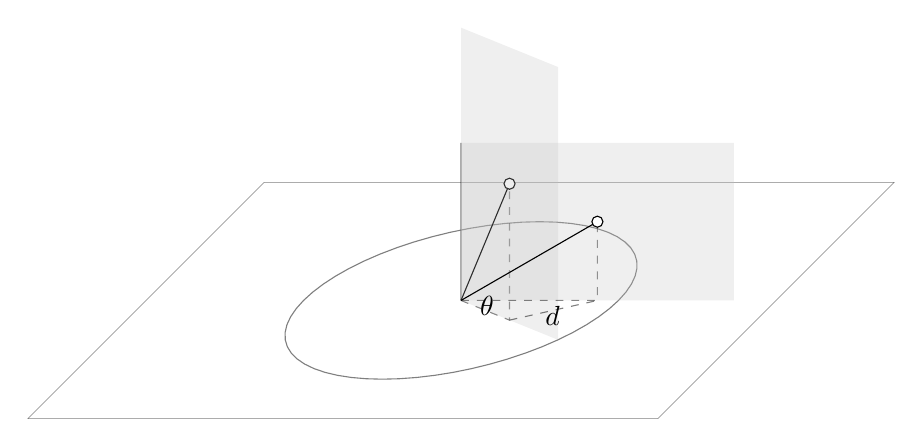
\begin{tikzpicture}[x={(1cm,0)},y={(-.5cm,-.5cm)},z={(0cm,1cm)}]% sistema di riferimento 3D
% piano di base
\draw [help lines](-4,-3,0)--(-4,3,0)--(4,3,0)--(4,-3,0)--cycle;

% draw base circle in plane xy and axis
\begin{pgfscope}
\pgfpathmoveto{\pgfpointorigin}
\pgfpathlineto{\pgfpointspherical{0}{90}{\maxdistance/2}}
\pgfpathmoveto{\pgfpointspherical{0}{0}{\maxdistance/2}}
\foreach\azimuth in {0,6,...,360} {
	\pgfpathlineto{\pgfpointspherical{\azimuth}{0}{\maxdistance/2}}
}
\pgfsetstrokeopacity{0.5}
\pgfusepath{stroke}
\end{pgfscope}

% draw for each target
\foreach \long/\lat/\distance in {60/60/2.,90/30/2} {
	\begin{pgfscope}
	% draw targets projection
	\pgfpathmoveto{\pgfpointorigin}
	\pgfpathlineto{\pgfpointspherical{\long}{0}{\distance*cos(\lat)}}
	\pgfpathlineto{\pgfpointspherical{\long}{\lat}{\distance}}
	\pgfsetstrokeopacity{0.5}
	\pgfsetdash{{1mm}{1mm}}{0pt}
	\pgfusepath{stroke}
	
	% draw azimutal plane
	\pgfpathmoveto{\pgfpointorigin}
	\pgfpathlineto{\pgfpointspherical{\long}{0}{\maxdistance*cos(\lat)}}
	\pgfpathlineto{\pgfpointspherical{\long}{\lat}{\maxdistance}}
	\pgfpathlineto{\pgfpointspherical{\long}{90}{\maxdistance*sin(\lat)}}
	\pgfpathclose
	\pgfsetfillcolor{lightgray}
	\pgfsetfillopacity{0.25}
	\pgfusepath{fill}
	\end{pgfscope}
	
	% draw target vector
	\begin{pgfscope}
	\pgfpathmoveto{\pgfpointorigin}
	\pgfpathlineto{\pgfpointspherical{\long}{\lat}{\distance}}
	\pgfsetstrokeopacity{1}
	\pgfusepath{stroke}
	\pgfpathcircle{\pgfpointspherical{\long}{\lat}{\distance}}{2pt}
	\pgfsetdash{}{0pt}
	\pgfsetfillcolor{white}
	\pgfsetfillopacity{1}
	\pgfusepath{fill,stroke}
	\end{pgfscope}
}
\pgfsetfillcolor{black}

% {60/60/2.,90/30/2}
\begin{pgfscope}
\pgfsetstrokeopacity{0.5}
\pgfsetdash{{1mm}{1mm}}{0pt}
\pgfpathmoveto{\pgfpointspherical{60}{0}{2*cos(60)}}
\pgfpathlineto{\pgfpointspherical{90}{0}{2*cos(30)}}
\pgfusepath{stroke}
\pgftext[right,at={\pgfpointspherical{75}{0}{1.5}}]{$d$}
\pgftext[right,at={\pgfpointspherical{75}{0}{.5}}]{$\theta$}
\end{pgfscope}
\end{tikzpicture}
\end{figure}

Per rilevare anche la quota del bersaglio è necessario utilizzare un altro \ac{RADAR} il cui fascio di radiazioni sia concentrato in un piano che ruoti trasversalmente al piano azimutale.

\clearpage
\section{Risoluzione geometrica radiale}\index{risoluzione geometrica radiale}
In presenza di più bersagli a distanze diverse per ogni impulso trasmesso il sistema \ac{RADAR} riceverà più segnali eco riflessi con attenuazioni e ritardi differenti. Le forme d'onda sono risolvibili l'una dall'altra fino a quando sono distinte all'uscita del filtro in ricezione, pertanto la capacità risolutiva è tanto maggiore quanto più stretta è la forma d'onda. L'uscita del filtro per un segnale sinusoidale sarà del tipo
\begin{equation}
s(t)=\intinf{S_R(f)\conj{S}(f)\e{\jmath\omega t_m}}{f}
\end{equation}
L'operazione del filtro è quella di calcolare l'autocorrelazione tra il segnale ricevuto e il modello del segnale inviato in modo tale da riconoscerlo. L'autocorrelazione di due segnali si può distinguere fino a quando è possibile distinguere gli spettri dei due segnali in uscita dal filtro adattato. Per un segnale rettangolare di periodo $T$ (o a inviluppo rettangolare) si ha per convoluzione un segnale triangolare di periodo $2T$: sarà possibile discriminare i due echi fino ad un ritardo temporale minimo pari a $\Delta T$, che corrisponde ad una capacità discriminatoria nello spazio pari a $\Delta R=c \Delta T/2$.

Per lo stesso motivo un sistema \ac{RADAR} ha una zona d'ombra entro la quale l'eco riflesso da un bersaglio torna prima che si sia terminato di trasmettere tutto il segnale di periodo $T$.

\begin{figure}[ht]\centering
\subfloat[Echi risolvibili]{
\begin{tikzpicture}
\begin{axis}[yscale=0.6,xlabel=$t$,ylabel=$s_T(t)$,xtick={1,2.5,4},xticklabels={$T$,$\tau_1$,$\tau_2$},ytick={-1,1},black,smooth,samples=300]
\def\omegazero{2*pi*8}
\addplot[domain=0:1] {sin((\omegazero*x))};
\addplot[domain=2.5:3.5] {.3*sin((\omegazero*x))};
\addplot[domain=4:5] {.25*sin((\omegazero*x))};
\end{axis}
\end{tikzpicture}
}\quad\subfloat[Echi sovrapposti]{
\begin{tikzpicture}
\begin{axis}[yscale=0.6,xlabel=$t$,ylabel=$s_T(t)$,xtick={1,2.5,3},xticklabels={$T$,$\tau_1$,$\tau_2$},ytick={-1,1},black,smooth,samples=300]
\def\omegazero{2*pi*8}\def\ampa{.3}\def \ampb{.25}
\addplot[domain=0:1] {sin((\omegazero*x))};
\addplot[domain=2.5:3] {\ampa*sin((\omegazero*x))};
\addplot[domain=3:4] {\ampa*sin((\omegazero*x))+\ampb*sin((\omegazero*x))};
\addplot[domain=4:4.5] {\ampa*sin((\omegazero*x))};
\end{axis}
\end{tikzpicture}
}
\caption{Schema segnale \ac{RADAR} trasmesso ed echi ricevuti}
\end{figure}

Per poter migliorare la risoluzione geometrica radiale è possibile ridurre la durata $T$ del segnale trasmesso, consentendo di discriminare echi con ritardi più vicini tra loro. Riducendo il periodo di trasmissione del segnale però si riduce l'energia trasmessa per cui è necessario amplificare il più possibile il segnale trasmesso.

In alternativa si può ottimizzare la capacità di riconoscere un segnale di durata molto breve ampliandone la banda trasmessa per ottenere una autocorrelazione quanto più stretta possibile: un segnale sinusoidale a frequenza crescente nel periodo $[0,T]$, detto \keyword[segnale!chirp]{chirp}. L'autocorrelazione di due segnali chirp sovrapposti ha carattere impulsivo di periodo $T_E=\frac{1}{B}$. La risoluzione radiale diventa non più funzione del periodo ma della banda del segnale trasmesso $\Delta R=\frac{c}{2B}$.

\begin{figure}[ht]\centering
	\begin{tikzpicture}
	\begin{axis}[yscale=.7,xlabel=$t$,ylabel=$s_T(t)$,xtick={1},xticklabels={$T$},ytick={-1,1},black,smooth,samples=500]
	\addplot[domain=0:1] {sin(((7*pi+32*pi*x)*x))};
	\end{axis}
	\end{tikzpicture}
	\caption{Segnale \textsc{Chirp}}
\end{figure}

\section{Bersagli fissi e mobili}
La conformazione del territorio attorno al \ac{RADAR} costituisce un bersaglio fisso il cui eco riflesso disturba la rilevazione di bersagli di interesse. Ad esempio un bersaglio aereo interposto tra l'antenna e una montagna (fig.~\ref{fig:radar_bersaglio_fisso}) sarà indistinguibile per il demodulatore ad inviluppo che rileverà un oggetto di sezione radar ordini di grandezza maggiore del bersaglio.

\begin{figure}[ht]\centering
	\begin{tikzpicture}[scale=.1]
	\draw (0,3) pic[rotate=35,scale=.5]{antenna} --++(-1,-3)--++(2,0)--++(-1,3);
	\draw [fill] (35:50) circle(10pt)node[left,outer sep=10pt]{bersaglio};
	\draw [decorate,decoration={expanding waves,angle=3}] (6,4)--(3,3.5);
	\draw [decorate,decoration={random,amplitude=10}](0,0)--(30,0)--++(60:50)--++(30:3)--++(-30:3)--++(-60:50)--++(0:5);
	\end{tikzpicture}
	\caption{Sistema \ac{RADAR} con bersaglio fisso}
	\label{fig:radar_bersaglio_fisso}
\end{figure}

Dato il segnale trasmesso $A\cos{\omega_0 t+\phi(t)}$ si riceverà con ritardi $\tau_1$ e $\tau_2$ la sovrapposizione degli echi della montagna e del bersaglio aereo:
\[\text{montagna}\colon\quad A_1\cos{\omega_0(t-\tau_1)+\phi(t-\tau_1)}=\Re{A_1\e{\jmath 2\pi\Phi_1}}\]
\[\text{bersaglio}\colon\quad A_2\cos{\omega_0(t-\tau_2)+\phi(t-\tau_2)}=\Re{A_2\e{\jmath 2\pi\Phi_2}}\]
\[A_R\cos{\omega_0 t-\phi_R(t)}\]

Per poter distinguere l'eco del bersaglio in movimento con $A_2\ll A_1$ si confronta non l'ampiezza dell'eco tra due scansioni successive ma la fase. L'ampiezza e la fase dell'eco della montagna risultano sostanzialmente costanti tra due scansioni successive dell'antenna in rotazione, mentre varierà la fase dell'eco del bersaglio mobile. Effettuando la differenza tra segnali ottenuti da due scansioni successive è possibile cancellare l'eco dei bersagli fissi e riuscire ad isolare l'eco del bersaglio in movimento (\ac{MTI}).

Per estrapolare la fase del segnale riflesso si utilizza un \keyword[demodulatore!I-Q]{demodulatore I-Q} con due portanti in quadratura.
\begin{figure}[h!]
	\centering
		\begin{tikzpicture}[>=latex',thick];
		\coordinate(c1);
		\coordinate[below=1cm of c1](c0);
		\coordinate[below=1cm of c0](c2);
		\node [left=1cm of c0](n0){$s_R$};
		\draw (n0)--(c0)|-(c1)(c0)|-(c2);
		\node [mult,right=1cm of c1](m1){} edge[<-](c1);
		\node [above=5mm of m1]{$2\cos{\omega_0 t}$} edge[->](m1);
		\node [passabasso,right=1cm of m1](pb1){} edge[<-](m1);
		\node [right=1cm of pb1]{$s_R^\text{I}$} edge[<-](pb1);
		\node [mult,right=1cm of c2](m2){} edge[<-](c2);
		\node [above=5mm of m2]{$2\sen{\omega_0 t}$} edge[->](m2);
		\node [passabasso,right=1cm of m2](pb2){} edge[<-](m2);
		\node [right=1cm of pb2]{$s_R^\text{Q}$} edge[<-](pb2);
		\end{tikzpicture}
	\caption{Schema di demodulatore I-Q in radar coerente}
	\label{fig:radar_demodulatore_IQ}
\end{figure}

Dato l'impulso \ac{RADAR} trasmesso $s_T(t)=\cos{\omega_0 t+\phi_T(t)}$ si suppone di ricevere il segnale riflesso sovrapposizione degli echi (ad es. della montagna e del bersaglio mobile) \[s_R(t)=a_R\cos{\omega_0 t+\phi_R(t)}=a_1\cos{\omega_0 (t-\tau_1)+\phi_R(t-\tau_1)}+a_2\cos{\omega_0 (t-\tau_2)+\phi_R(t-\tau_2)}\]
che in ingresso al demodulatore I-Q in modulazione con le portanti in quadratura danno
\[s_R^\text{I}(t)=a_R\cos{\omega_0 t+\phi_R(t)}\cdot 2\cos{\omega_0 t}=a_R\cos{\phi_R(t)}\]
\[s_R^\text{Q}(t)=a_R\cos{\omega_0 t+\phi_R(t)}\cdot 2\sen{\omega_0 t}=a_R\sen{\phi_R(t)}\]

Dai segnali in fase e quadratura si può ricavare l'ampiezza e la fase del segnare ricevuto:
\[a_R(t)=\sqrt{s_R^\text{I}(t)^2+s_R^\text{Q}(t)^2}\quad\phi_R(t)=\arctan\frac{s_R^\text{Q}(t)}{s_R^\text{I}(t)}\]

Tra due scansioni successive posso avere inviluppi di ampiezza simili ma è possibile apprezzare i cambiamenti di fase essendo
\[\Phi_R(t)=\Phi_1(t)+\arctan\frac{a_2\sen{\Phi_2-\Phi_1}}{a_R}\]

\[			\begin{split}\Phi_R''-\Phi_R'=\phi_R''-\phi_R'&=-\arctan\frac{a_2'\sen{\Phi_2'-\Phi_1}}{a_R'}+\arctan\frac{a_2''\sen{\Phi_2''-\Phi_1}}{a_R''}=\\
&\cong\frac{a_2''\sen{\Phi_2''-\Phi_1}-a_2'\sen{\Phi_2'-\Phi_1}}{a_1}\quad(a_1\gg a_2\implies a_R=a_1)\end{split}\]

\begin{figure}[!ht]\centering
	\begin{tikzpicture}[>=latex',black,scale=.9]
	\draw[<->](0,4)node[above]{$\Imaginarypart$}--(0,0)--(6,0)node[right]{$\Realpart$};
	\coordinate (O) at (0,0);
	\coordinate (A) at (30:5);
	\coordinate (B) at ($(A)+(60:1.5)$);
	\coordinate (C) at ($(A)+(30:1.5)$);
	\coordinate (D) at ($(A)+(120:1.5)$);
	\coordinate (E) at (3,0);
	\coordinate (F) at (5,0);
	\draw[thick,->](O)--node[below]{$a_1$}(A);
	\draw[thick,->](A)--node[pos=0.99,right]{$a_2$}(B);	
	\draw[thick,->](O)--node[above]{$a_R$}(B);
	\draw[thin] (A)--(C);
	\draw[thin] (E)--(B);
	\draw[thin] (1,0) arc(0:30:1) node[pos=.5,right]{$\Phi_1$};
	\draw[thin] (4,0) arc(0:60:1) node[pos=.5,right]{$\Phi_2$};
	\draw[thin] ($(A)+(30:1)$) arc(30:60:1) node[pos=.66,right]{$\Phi_R$};
-	\end{tikzpicture}
	\caption{Fasori segnale modulato in quadratura}\label{fig:segnale_modulato_in_quadratura}
\end{figure}

In un breve intervallo di tempo tra due scansioni il bersaglio si sarà spostato di poco pertanto è possibile approssimare il seno dell'angolo con l'angolo
\[\Phi_R(t)\cong\Phi_1(t)+\frac{a_2}{a_1}(\Phi_2-\Phi_1)\]
\[\begin{split}\Delta\Phi_R&=\frac{a_2}{a_1}\Delta\Phi=\frac{a_2}{a_1}\left[\underbrace{(\omega_0 t-\omega_0\tau_2''+\phi_T(t-\tau_2''))}_{\Phi_2''}-\underbrace{(\omega_0 t-\omega_0\tau_2'+\phi_T(t-\tau_2'))}_{\Phi_2'}\right]=\\
&=\frac{a_2}{a_1}[\omega_0 (\tau_2''-\tau_2'')+\phi_T(t-\tau_2'')-\phi_T(t-\tau_2')]\end{split}\]


\clearpage
\section{Shift Doppler}
Il sistema \ac{RADAR} può rilevare se il bersaglio in movimento è in avvicinamento o allontanamento sulla congiungente antenna-bersaglio. Si determina la distanza radiale $v_R$ del bersaglio in movimento, considerando costante la velocità radiale nell'intervallo tra due impulsi radar:
\begin{equation}
R(t)=R_0+v_R t
\end{equation}

Il tempo necessario al segnale di propagarsi, riflettersi sul bersaglio e tornare indietro diventa una funzione del tempo
\begin{equation}
\tau(t)=\frac{2 R(t)}{C}=2\frac{R_0+v_R t}{c}=\tau_0+k t\quad k=\frac{v_R}{c}
\end{equation}

Il segnale riflesso subisce un ritardo tempovariante $s_R(t)=s_T(t-\tau_0-k t)$ ha spettro per la trasformata di Fourier
\[S_R(f)=\intinf{s(t-\tau_0-k t)\e{-\jmath 2\pi f t}}{f}\]
effettuando il cambio di variabile $\alpha=t-\tau_0-k t$, $t=\frac{\alpha+\tau_0}{1-k}$, $\diff t=\frac{\diff\alpha}{1-k}$,
\[\begin{split}S_R(f)&=\intinf{\frac{s(\alpha)}{1-k}\e{-\jmath 2\pi f\left(\frac{\alpha}{1-k}+\frac{\tau_0}{1-k}\right)}}{\alpha}=\\
&=\frac{\e{-\jmath 2\pi f\frac{\tau_0}{1-k}}}{1-k}\intinf{s(\alpha)\e{-\jmath 2\pi f\frac{\alpha}{1-k}}}{\alpha}=\\
&=\frac{\e{-\jmath 2\pi f\frac{\tau_0}{1-k}}}{1-k} S\left(\frac{f}{1-k}\right)\end{split}\]

Si può notare che la singola componente sinusoidale dello spettro moltiplicata per l'operatore lineare ritardo, che ha funzione di trasferimento $\e{-\jmath\omega\tau}=\e{-\jmath 2\omega\frac{R_0}{c}}\e{-\jmath 2\omega\frac{v_R}{c}t}$, risulta variata nell'ampiezza e ruotata nella fase: alla frequenza $f_A$ corrisponde la $\frac{1}{1-k}f_A$, con una variazione $\Delta f=f_A-\frac{f_A}{1-k}=\left(1-\frac{1}{1-k}\right)f_A=\frac{-k}{1-k}f_A\cong-k f_A=-\frac{v_R}{c}f_A$

Un segnale passa banda stretta avrà il centro banda $f_0$ traslato in $f_0-\frac{v_R}{c}f_0$, e l'estremo $f_\text{min}$ in $f_\text{min}-\frac{v_R}{c}f_\text{min}$
\begin{figure}[ht!]\centering
	\def\fmin{500.}\def\fmax{3000.}
	\def\fmina{450.}\def\fmaxa{2700.}
	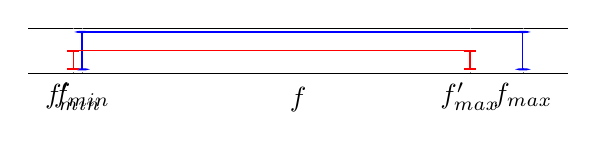
\begin{tikzpicture}
	\begin{axis}[hide y axis,yscale=.1,xlabel=$f$,extra x ticks={\fmina,\fmaxa,\fmin,\fmax},xtick={100,10000},extra x tick labels={$f_\text{min}'$,$f_\text{max}'$,$f_\text{min}$,$f_\text{max}$},extra x tick labels/.style={inner sep=10pt},domain=10:10000,every x tick scale label/.style={at={(xticklabel* cs:.9,5pt)},/pgfplots/near ticklabel align=outside,anchor=near xticklabel opposite,inner sep=0pt},]
	\addplot coordinates {(\fmin,0)(\fmin,1)(\fmax,1)(\fmax,0)};
	\addplot coordinates {(\fmina,0)(\fmina,.5)(\fmaxa,.5)(\fmaxa,0)};
	\end{axis}
	\end{tikzpicture}
\end{figure}
